%% -*- coding: utf-8 -*-
\documentclass{article}
% Outline for statistics tutorial
% Hal Canaray and Cory Quammen
\usepackage{graphicx}
\usepackage{utfsymb}
\begin{document}

\begin{center}
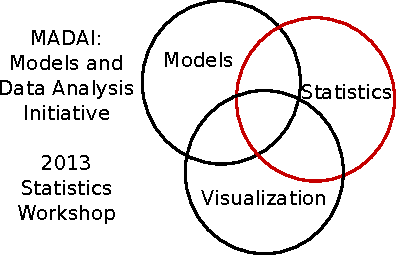
\includegraphics{figures/MADAI_2013_Stats_Workshop.pdf}
\end{center}

\section{Statistics background}

\subsection{Basic concepts}

We have a model and we're trying to find parameters for it that best
explain some observed phenomena.

\begin{itemize}

\item Model — a conceptual model of a physical process.  It exists as
  a procedure that takes in parameters and returns either a set of
  outputs or a distribution of outputs.

\item Observables — a set of field measurements that can be compared
  against a model's outputs.

\item Output Space — The set of all possible outputs of the model,
  which are intended to be comared to observations.

\item Model Outputs — a point in output space, or a distribution in
  output space.

\item Model Parameters — any of the modifiable inputs to the model

\item Parameter Space — the set of all possible values for each of the
  parameters

\item Ground Truth — a point in parameter space that represents how
  the universe actually works.  Will only exist if the model is any
  good..

\item Likelihood — Given a model and set of observables, what is the
  probability of a given set of parameter values?  What we actually
  calulate is the likelihood ratio.

\end{itemize}

\begin{center}
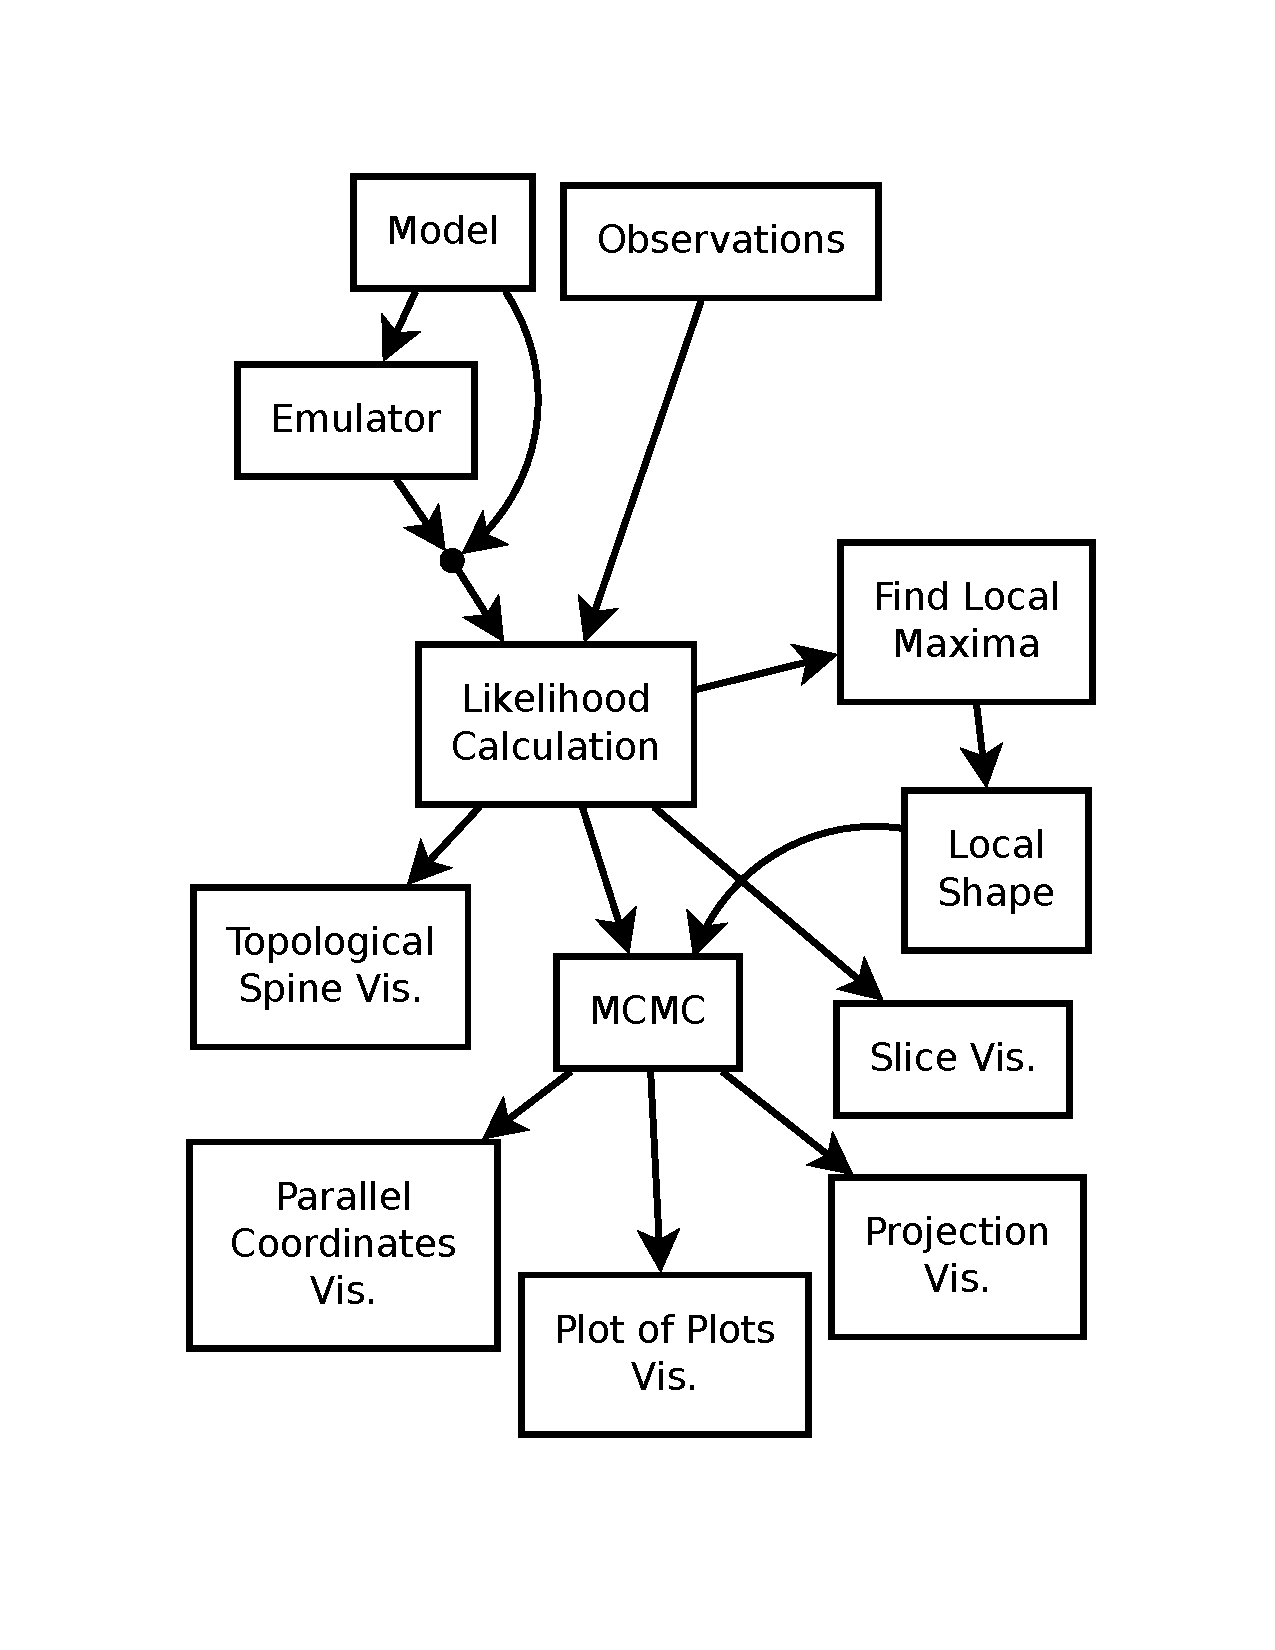
\includegraphics[width=3in]{figures/MADAI_Stats_and_Vis.pdf}
\end{center}


\subsubsection{Probability and statistics review}

Touch on terms.

Probability, expectation, distribution, joint distribution, variance,
covariance

\subsubsection{Joint implausbility}

\section{Gaussian process emulator}

\subsection{Background}

See Chris Coleman-Smith's presentation at the June 2012 MADAI meeting on this

\begin{itemize}

\item What it does?

\item Why use it instead of interpolation?

\item How to use it?

\end{itemize}

\subsection{Training an emulator}

\subsubsection{What is a nugget?}

\subsubsection{Inputs}

\begin{itemize}

\item Set regression order - this subtracts a broad trend in the data to make the training better behaved

\item Pick a covariance function - this is a kernel that determines the weights of nearby training data on an output

\item PCA variance (0.0 - 1.0) - how much of the variance do you want to explain?

\end{itemize}

\subsection{Verify emulator}

Feed training points back into emulator. Results won't be identical, but should be close. Jittering parameter-space position should give you similar values.

\section{Markov Chain Monte Carlo}

\subsection{Background}

\subsection{Algorithm we use}

Metropolis-Hastings

\subsection{Burn-in}

\subsection{Post burn-in}



\section{Software session}

\subsection{Download code}

\subsubsection{MADAI Workbench}

\subsubsection{Emulator}

Set up environment for running it

\subsubsection{Data}

\begin{itemize}

\item One die example data in format useful for training. Question: How long is this going to take?

\item Two die example

\end{itemize}

\end{document}
